\chapter{Conclusion}
\label{sec:conclusion}

\ifpdf
    \graphicspath{{10_conclusion/figures/PNG/}{10_conclusion/figures/PDF/}{10_conclusion/figures/}}
\else
    \graphicspath{{10_conclusion/figures/EPS/}{10_conclusion/figures/}}
\fi

Particle detectors are often the source for studying and collecting data in particle physics. These instruments gather exabytes of data that need to be thoroughly probed for relevant signals. While the state-of-the-art in hardware has significantly improved and allowed for detailed data collection, traditional physics controls are often unable to keep up with the large, high dimensional, irregular data. With this gap between information extraction techniques and information gathering systems, attention has shifted to artificial intelligence. Research is required to explore the feasibility of state-of-the-art architectures to particle data before they can be incorporated into the processing pipeline. This thesis examined one such state-of-the-art deep learning architecture - PointNet, and its ability to learn from 3D mesh representation of neutrino data.

The goal of the thesis was to build a classification network that could label a timeslice as \texttt{0} or \texttt{1}, such that noise could be discarded and events could be saved. The three research questions were revisited based on the results from the thesis. In order to answer \textbf{RQ1.0} and \textbf{RQ 1.1}, \textbf{RQ 2.0} and \textbf{RQ 2.1} were first resolved. 

\begin{description}
    \item[\textbf{RQ2.0}] \textit{Can the KM3NeT dataset be effectively represented using 3D meshes?} \\
    3D mesh representations of the feature engineered point clouds demonstrated that meshes are a valid representation of the KM3NeT data. Moreover, secondary experiments that used 3D and 4D point clouds showed insufficient learning through means of low precision and recall scores (Section \ref{sec:additional}). 3D meshes likely outperformed point-based learning because the meshes added more information to the point clouds in the form of mesh faces and normals. Moreover, PointNet requires a fixed number of points to be randomly sampled per point cloud. With 3D meshes, the thesis was able to sample per mesh face, retaining much of the shape of the data. 
    
    \item[\textbf{RQ2.1}] \textit{Which meshing algorithm would be most suitable for representing the data?}  \\
    Poisson Surface Reconstruction was found to be most suitable for representing KM3NeT data. Based on visual examinations, it showed greater detail, especially around event clusters (Section \ref{sec:pipeline}). It was however not able to capture details in timeslices with few event hits. Ball-Pivoting Algorithm was also used to reconstruct point clouds. While BPA was found to be significantly faster in building meshes, it was too simplistic for the detailed event clusters (Section \ref{sec:pipeline}). 
    
    \item[\textbf{RQ1.0}] \textit{Can PointNet, a geometric Neural Network architecture be trained to classify timeslices that contain neutrino event hits from timeslices that contain only background noise?} \\
    PointNet can be successfully trained to classify timeslices of the KM3NeT data. This was indicated via high recall scores for the positive class and the Precision-Recall curves, measured via Hard Voting (Section \ref{sec:results}). It also outperformed the existing L1 Trigger, which had a higher false positive rate. However, PointNet was not able to correctly classify timeslices with events containing a few hits, for example 30 to 40 event hits. 
    
    \item[\textbf{RQ1.1}] \textit{Can PointNet achieve a Precision-Recall score of greater than 0.9 for identifying timeslices with event hits?} \\
    Hard-voting predicted a 0.95 recall and perfect precision scores for  \texttt{class\_1} containing event hits. Therefore, it met stakeholder expectations. However, it was only able to do so with feature engineering and mesh representations. Without feature engineering, it was unable to learn between classes (Appendix \ref{appendix}), and without meshes, it scored no more than 0.70 on recall and precision (Section \ref{sec:additional}). 
     
    \item[\textbf{RQ3.0}] \textit{Can PointNet be extended to obtain energy properties from neutrino events?} \\
    The thesis does not recommend extending PointNet for regression tasks. As PointNet is built for classification, it would require several changes to make it suitable for regression. Further, mapping the energy values to the completely randomised and transformed point clouds after classification tasks would be inefficient. Experiments are instead conducted using random forests. The trained model can predict a minimum energy of 12.138 GeV for events containing 32 hits.

\end{description}

The pipeline in Figure \ref{fig:complete_pipeline} was the finalised thesis pipeline. Three permutations of the KM3NeT dataset were obtained and processed using radius-based outlier filter. They were then converted to 3D meshes and trained using PointNet. Several transformation functions were applied to the data during training and testing. Majority voting was used to ensemble results and obtain final output.

\begin{figure}[ht!]
    \centering
    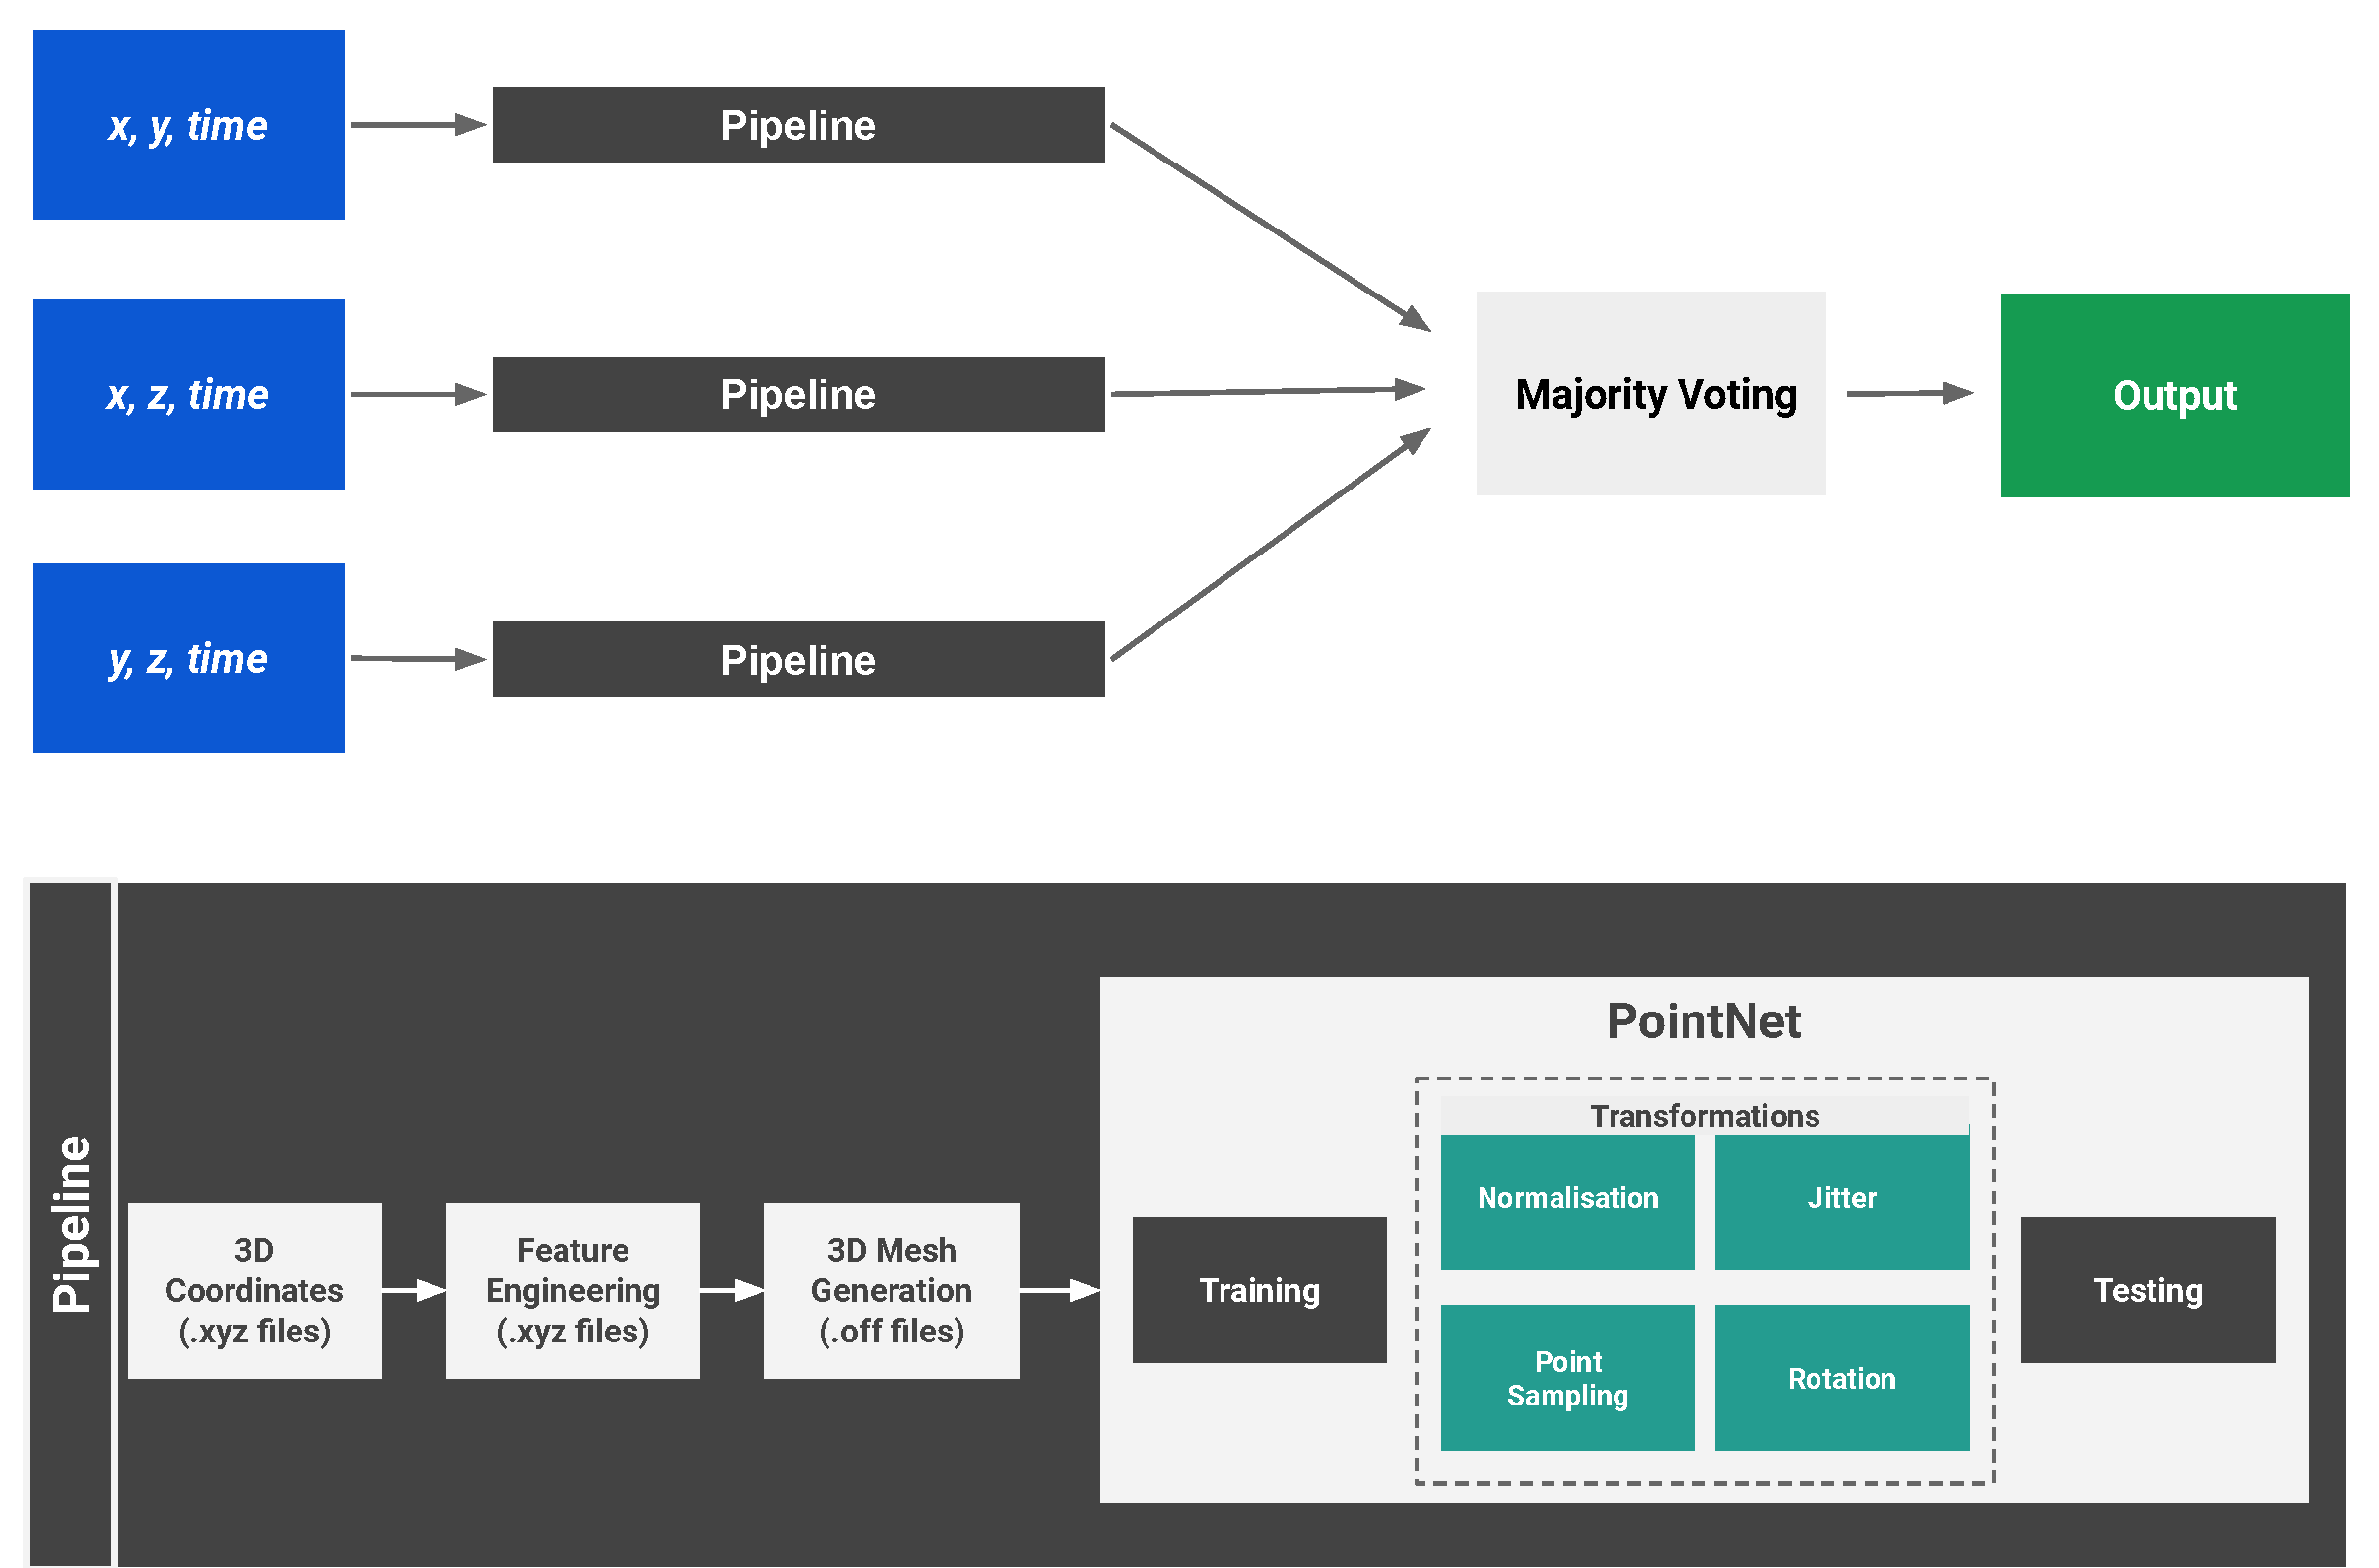
\includegraphics[width=0.8\textwidth,height=7cm,keepaspectratio]{complete_pipeline.pdf}
    \caption{The Complete Process for KM3NeT Timeslice Classification}
    \label{fig:complete_pipeline}
\end{figure}

Despite the noted limitations, this thesis lays the groundwork for 3D point-based deep learning for neutrino identification amidst noise. The thesis is the first known application of 3D point-based learning for neutrino detection. It is also the first known work to use 3D meshes to represent neutrino data and achieve high precision and recall scores. 

Results from this thesis can be used by physicists at KM3NeT to assess the feasibility of adopting PointNet into the pipeline. They could also extend the architecture to classify the three neutrino flavours \cite{km3net_2017}. The event trigger is an important aspect of the KM3NeT pipeline, both from a fiscal and physics perspective as it determines data that needs to be saved or discarded \cite{km3net_2017}. The methodology developed in this thesis demonstrates a high recall and low false-positive rate. Thus, making use of this as a KM3NeT pipeline would both minimise the noise being saved and ensure that timeslices with events are saved with a high accuracy. Results from this thesis can also help ascertain the validity of novel point-based learning for particle physics data. The methods undertaken, the problems faced and the results obtained could serve as a starting point for others in particle physics wishing to adopt Neural Networks to their own work.

While this thesis serves as a starting point for examination of novel deep learning architectures for neutrino research, there is certainly more work required to understand how complex networks could be tuned to meet the end goals in the field. Additional studies would be required to understand performance of the pipeline on the GPU. Adopting deep learning always presents a trade-off between superior accuracy of results and longer compute times. These trade-offs would require careful examination against existing methodology. Despite these gaps, PointNet at its current state has a very promising role in the future of neutrino research and by extension particle physics.

\let\cleardoublepage\clearpage



